211. \begin{figure}[ht!]
\center{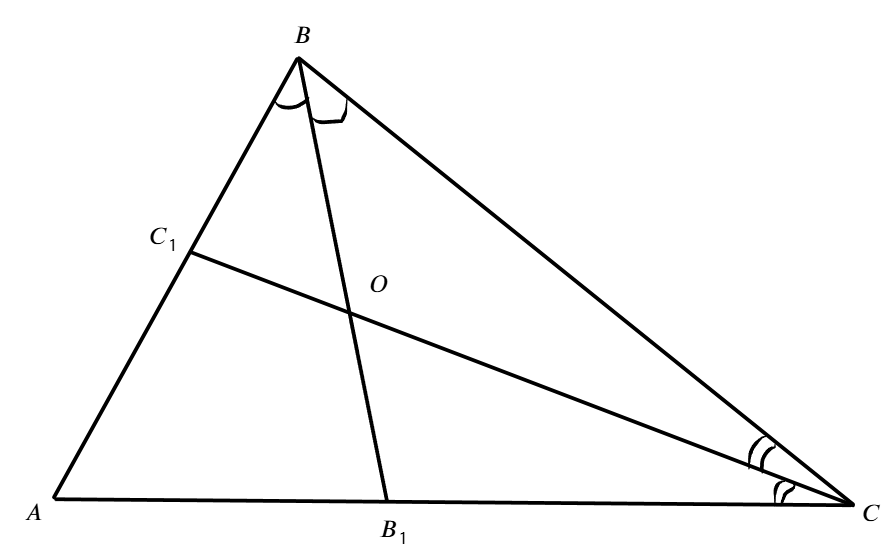
\includegraphics[scale=0.35]{g9-206.png}}
\end{figure}\\
По свойству основания биссектрисы для треугольника $ABC$ имеем соотношение
$\cfrac{BC_1}{AC_1}=\cfrac{BC}{AC}=\cfrac{5}{7},$ при этом $AC_1+BC_1=AB=3,$ откуда $AC_1=\cfrac{7}{12}AB,\ BC_1=\cfrac{5}{12}\cdot3=\cfrac{5}{4}.$ Тогда $\overline{CC}_1=\overline{CA}+\overline{AC}_1=-\vec{c}+\cfrac{7}{12}\vec{b}.$
По свойству основания биссектрисы для треугольника $BC_1C$ имеем соотношение
$\cfrac{CO}{OC_1}=\cfrac{BC}{BC_1}=\cfrac{5}{\cfrac{5}{4}}=4,$ а значит $CO+\cfrac{1}{4}CO=CC_1,\ CO=\cfrac{4}{5}CC_1.$ Таким образом, $\overline{CO}=\cfrac{4}{5}\cdot\left(-\vec{c}+\cfrac{7}{12}\vec{b}
ight)=
\cfrac{7}{15}\vec{b}-\cfrac{4}{5}\vec{c}.$
ewpage
oindent
